\documentclass[10pt,a4paper]{article}
\usepackage[margin=14mm]{geometry}
\usepackage[T1]{fontenc}
\usepackage{lmodern}
\usepackage{graphicx}
\usepackage{xcolor}
\definecolor{accent}{HTML}{235D69}
\definecolor{ink}{HTML}{202B35}
\usepackage{enumitem}
\usepackage{titlesec}
\usepackage{hyperref}
\hypersetup{colorlinks=true,urlcolor=accent,pdftitle={Pierre Guilbert - Curriculum Vitae},pdfauthor={Pierre Guilbert}}
\pagestyle{empty}
\setlength{\parindent}{0pt}
\setlength{\parskip}{3pt}
\setlist[itemize]{leftmargin=12pt,itemsep=1pt,topsep=2pt,parsep=0pt}
\titleformat{\section}{\sffamily\large\color{accent}}{}{0pt}{}[\vspace{3pt}\titlerule]
\titlespacing*{\section}{0pt}{8pt}{5pt}
\newcommand{\entry}[2]{\textbf{#1}: #2\par}
\begin{document}
\color{ink}
\begin{minipage}[t]{0.80\textwidth}
\vspace{0pt}
{\sffamily\fontsize{27}{30}\selectfont Pierre Guilbert}\par
{\sffamily\color{accent} Computer Vision, Machine Learning \& Mathematical Modelling}\par

Saint-Sulpice, Switzerland\par \href{mailto:spguilbert@gmail.com}{spguilbert@gmail.com} \enspace | \enspace \href{tel:+41786576581}{+41 78 657 65 81}\par
\href{https://github.com/PierreGuilbertF?tab=repositories}{GitHub} \enspace | \enspace \href{https://www.linkedin.com/in/pierre-guilbert}{LinkedIn}\par\vspace{3pt}
\end{minipage}\hfill
\begin{minipage}[t]{0.16\textwidth}
\vspace{0pt}
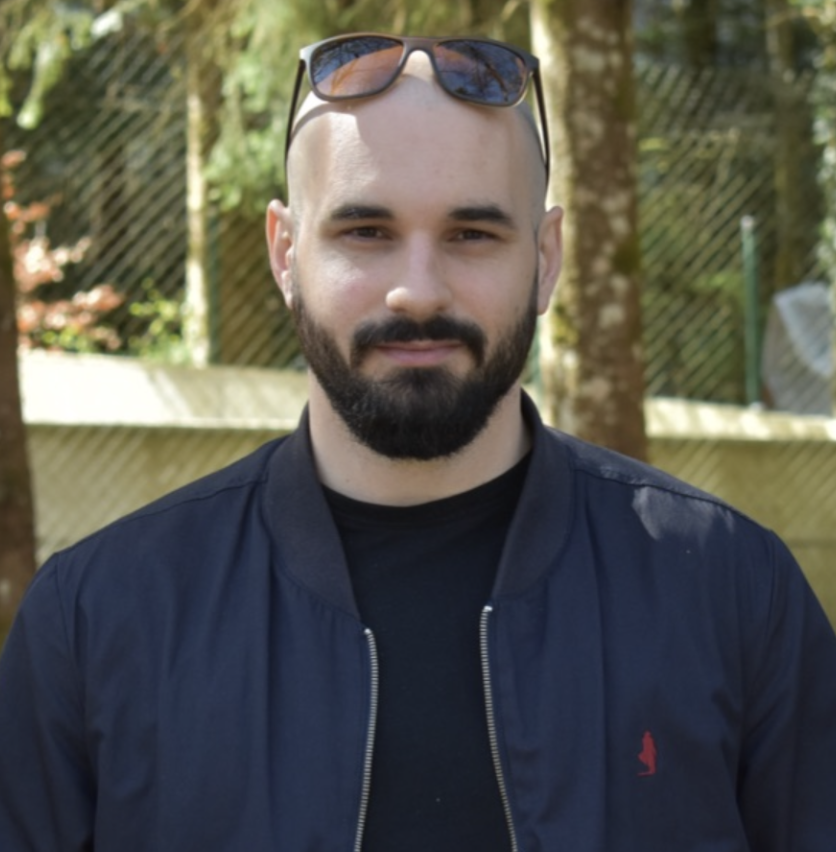
\includegraphics[width=\linewidth]{profile_picture.png}
\end{minipage}\par\vspace{5pt}
Engineer with 10 years of experience in Computer Vision, Machine Learning, and Mathematical Modelling, with a strong interest in differential geometry and nonlinear optimization.\par
Passionate about applying advanced mathematics to real-world challenges, I enjoy combining technical expertise and creative problem-solving through collaboration and intellectual exchange.\par
\section{Experience}
\textbf{Genius Sports} --- Senior Computer Vision Engineer\hfill {\small 2019 - Present}\par
{\small\itshape Lausanne}\vspace{-3pt}
\begin{itemize}
\item Camera modelling and calibration: keypoint detection, bundle adjustment, and optical SLAM.
\item Human pose estimation: body keypoint detection, triangulation, and trajectory optimization based on physical laws and optical measurements.
\item Geometric and physical parameter estimation from multi-view images: 3D reconstruction, Gaussian splatting, ball spin, and ball deformation.
\item Ad-tech: auction price optimization and user click-through prediction.
\end{itemize}
\textbf{Kitware} --- Computer Vision Engineer\hfill {\small 2016 - 2019}\par
{\small\itshape Lyon}\vspace{-3pt}
\begin{itemize}
\item Software engineering for VeloView: lidar, multi-sensor fusion, and point-cloud processing.
\item Lidar-based SLAM: design and implementation of a lidar-based SLAM system inspired by the LOAM algorithm.
\item Contributions to open-source projects: VTK, ParaView, and Ceres Solver.
\end{itemize}
\textbf{CNRS} --- Image Processing Research Assistant\hfill {\small 2015 - 2016}\par
{\small\itshape Saint-Étienne}\vspace{-3pt}
\begin{itemize}
\item Research in image and signal processing using the logarithmic image processing (LIP) model.
\item Neural network training framework using LIP operations.
\end{itemize}
\section{Skills}
\entry{Mathematical Modelling}{Physics, PDEs, variational calculus, nonlinear optimization}
\entry{Computer Vision}{Multi-view geometry, bundle adjustment, SLAM, pose estimation}
\entry{Machine Learning}{Design and training of discriminative and generative models (classification, segmentation, regression, density estimation) with PyTorch}
\entry{Mathematics}{Differential geometry, topology, measure theory, algebra}
\entry{Programming}{C++ (Eigen, Ceres, OpenCV, PCL), Python, Git}
\section{Education}
\textbf{Graduate studies in Mathematics \& Engineering} --- Mines Saint-Étienne\hfill 2016\par
\textbf{MSc Computer Graphics \& Signal Processing} --- Université Lyon 1\hfill 2015\par
\textbf{MEng Electrical Engineering} --- Université Lyon 1\hfill 2015\par
\textbf{BSc Mathematics, Physics \& Chemistry} --- CPGE Champollion\hfill 2012\par
\section{Personal Interests}
\entry{Philosophy \& Literature}{Exploring morality, ethics, consciousness, and the nature of reality}
\entry{Stock market investment}{Long-term stock picking with no intention to outperform the market, but to learn from it}
\entry{Powerlifting}{Strength training in bench press, deadlift, and squat}
\entry{Mathematics}{Exploring the state of the art, writing research notes and short mathematical treatises}
\end{document}
